\documentclass[journal]{IEEEtran}

% *** CITATION PACKAGES ***
\usepackage[style=ieee]{biblatex} 

\usepackage{url}
% correct bad hyphenation here
\hyphenation{op-tical net-works semi-conduc-tor}
\usepackage{graphicx}  %needed to include png, eps figures
\usepackage{float}  % used to fix location of images i.e.\begin{figure}[H]
\usepackage{times}
\usepackage{authblk}
\usepackage{epsfig}
\usepackage{wrapfig}
\usepackage{graphicx}
\usepackage{amsmath}
\usepackage{amssymb}
\usepackage[english]{babel}
\usepackage{graphicx}
\usepackage{times}
\usepackage{epsfig}
\usepackage{graphicx}
\usepackage{amsmath}
\usepackage{amssymb}
\usepackage{array}
\usepackage{authblk}
\usepackage{blindtext}
\usepackage{float}
\usepackage[english]{babel}
\setcounter{page}{1}
\usepackage{dblfloatfix}    % To enable figures at the bottom of page
\usepackage[breaklinks=true,bookmarks=false]{hyperref}

\def\httilde{\mbox{\tt\raisebox{-.5ex}{\symbol{126}}}}
\setcounter{page}{1}
\begin{document}

\title{Optimizing Precision Genome Editing through Machine Learning}


\author{Shi-an Anderson Chen \textsuperscript{1}\thanks{\noindent\textsuperscript{1} Department of Biology}, Elizabeth Tran \textsuperscript{2}\thanks{\noindent\textsuperscript{2} Department of Biomedical Informatics and Department of Psychiatry and Behavioral Science}  \\
Stanford University \\
{\tt\small { eliztran, shian @stanford.edu}}\\
}
\maketitle

%%%%%%%%% ABSTRACT
\begin{abstract}
Precision genome editing opened the door to better understand the impact of genetics on living organisms by analyzing the underlying genetic blueprints. One critical system supporting precision genome editing is CRISPR-Cas9, which provides scalable targeted cleavage of DNA through guide RNA programming. Thus, prediction and minimizing of off-target cleavage effects of CRISPR-Cas9 is a crucial research area to improve efficacy of genome editing technology. This paper discusses our analysis of the off-target effects based on several hyper parameters used in CRISPEY, a novel high-throughput precision gene editing approach leveraging CRISPR-Cas9, in order to improve off-target prediction performance. After applying several machine learning algorithms and a simple deep neural network (DNN), we identified a relatively high performing support vector machine (SVM) model with a 64$\%$ recall rate. This model allows us to predict potential off-target guide RNAs in precision gene editing studies and through the exclusion of such suboptimal guide RNAs we can circumvent false negative readout post-editing, ultimately reduce experimental noise and reagent cost in CRISPEY experiments.
\end{abstract}
%%%%%%%%% BODY TEXT

\section*{Introduction}
Genetic variation is key to successful adaptive evolution: genotype changes can lead to changes in phenotype and thus individual fitness. By better identifying the consequences and impact of genetic variations, we can gain insight into understanding how such variation impact health in both positive and negative ways. The introduction of new gene editing techniques such as CRISPR  (clustered regularly interspaced short palindromic repeats)-Cas9 have allowed scientists to study genetic variations in greater detail. CRISPR-Cas9 introduces precise changes to an individual  genome by programming molecules called guide RNAs. The Cas9 protein carries the guide RNA to the target genomic region where it breaks apart the DNA and replaces it with an alternate DNA template supplied by the CRISPR guide RNA. Once the alternate has replaced the original, the edited target can be assayed for phenotype. If the phenotype exhibits new behavior from the replacement, we can infer that the alternate gene is responsible. The simplicity and effectiveness of CRISPR-Cas9 has led to it becoming a popular tool to study genetic variants and has provided an exciting new opportunity to use the CRISPR-Cas9 as a therapeutic treatment by supplying healthy alternative  gene variations.

Off-targeting is a phenomenon caused when the Cas9 protein introduces double-stranded breaks to DNA where the guide RNA does not match, resulting in unintended changes in the genome and negating any causal inference that could be drawn from the experiment. Even worse, if used for therapy, 
\begin{figure}[h]
	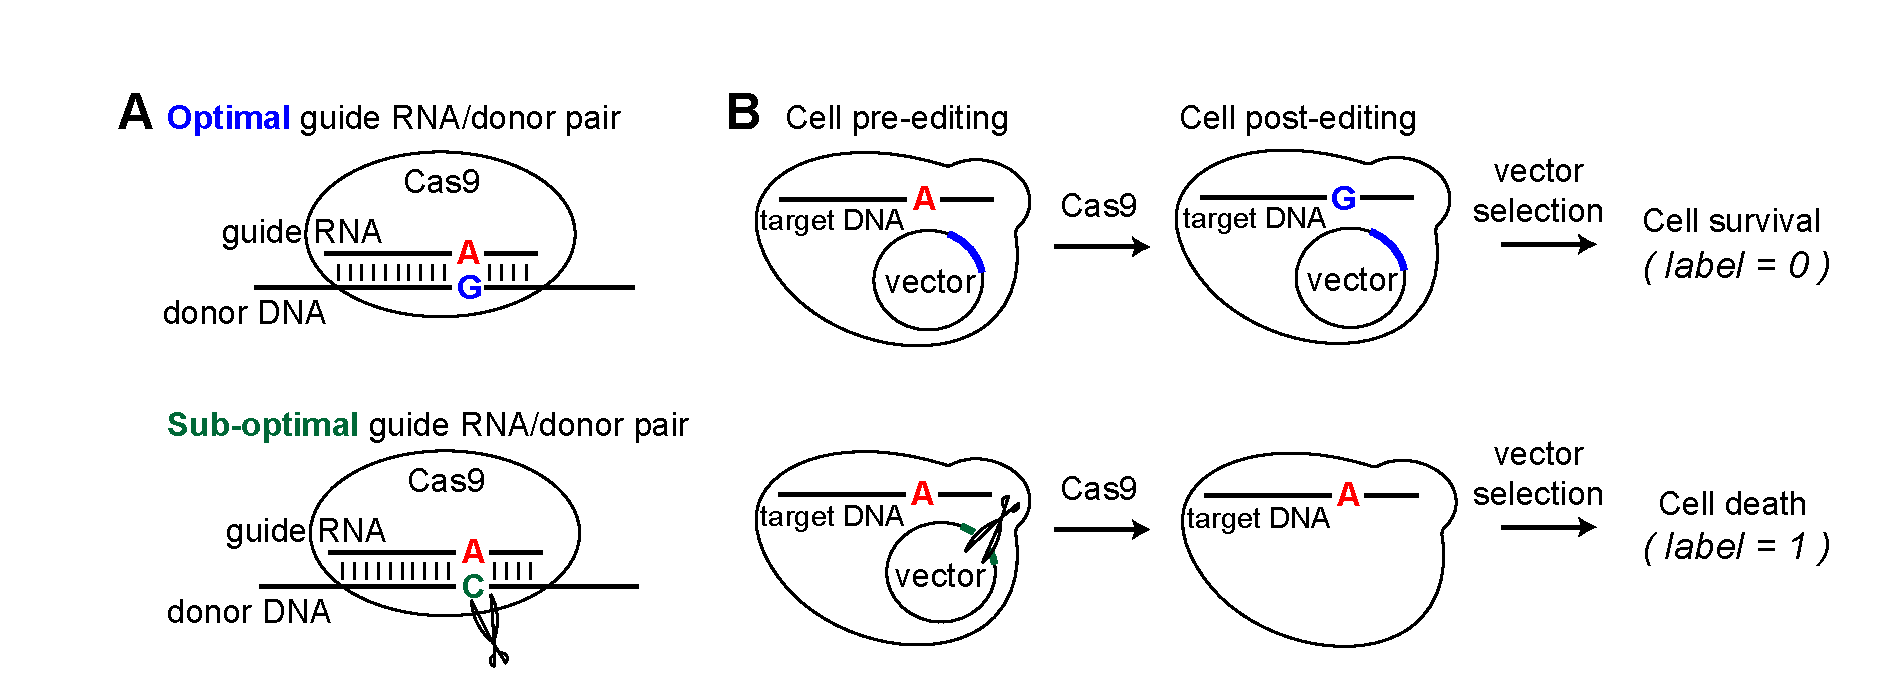
\includegraphics[width=10cm]{../self_cut}
	\caption{Optimal vs. Suboptimal guide RNA/donor DNA pairs during CRISPEY editing}
\end{figure}  off-targeting could introduce potentially fatal and unpredictable mutations. To improve guide RNA selection, we need to develop more effective prediction models and improve our understanding of specific RNA features. The application of machine learning can play a role in classifying off-target prone guide RNAs, allowing us to select the best guide RNAs to be used in research and therapeutics. 


\section*{Related Works}
Fields like protein structure prediction, homology modeling and cheminformatics frequently employ tools from machine learning, such as PCA, dimensionality reduction, SVMs (Support Vector Machine), clustering, random forest (RF) classifier, etc. With the advent of deep neural networks (DNN), there have been groundbreaking improvements in feature representation (Krizhevsky et al., 2012), object classification, and pattern recognition (He et al., 2016). DNNs utilize stacked layers of nonlinear operations instead of manually extracting features from input data and its multi-layers learning can get a more effective expression. However, there have not been many deep learning applications for CRISPR-Cas9 off-target prediction (Chuai et al., 2018; Lin \&\ Wong, 2018). The current methods that have been proposed have used a variety of machine learning algorithms. Even though they seem promising, the models are not necessarily generalizable.
CRISPEY (Cas9 retron precise parallel editing via homology), a novel genome-editing technique developed at Stanford in 2018, empirically measures in parallel the fitness effects of thousands of natural genetic variants in yeast at single-base resolution. This editing approach was able to discover hundreds of variants affecting fitness, giving us enough statistical power to show that these variants are enriched for genomic features such as promoters and transcription factor (TF) binding sites. Unexpectedly, the study also generated data on off-target effects for the thousands of guide RNAs that are used for variant editing, empirically measured by cellular toxicity during editing. In the yeast cell, co-introduction of donor DNA and guide RNA on the same vector meant that suboptimal guide RNA/donor DNA pairs will lead to cutting of the donor DNA by Cas9, which is observed in the editing phase of CRISPEY experiments (Fig. 1A). Such guide RNA/donor DNAs lead to self-destruction of editing vector and subsequently cell death, providing no information about the edit and waste of experimental throughput (Fig. 1B) This data set is a rich resource for modeling off-target effect with thousands of guide RNAs, compared to previous studies that typically only look at most a few dozen guide RNAs. Here, we explore a variety of machine learning techniques to model the CRISPEY dataset, with the goal to predict reliable guide RNAs that are less prone to off-targeting. By extracting features that are predictive of guide RNA off-target activities will help us learn about the sequence to function relationship of guide RNAs that CRISPR-Cas9 activity is dependent on. Lastly, the obtained model will be useful for setting up a framework for evaluating other genome editing tools that use sequence-dependent, programmable DNA nucleases other than Cas9. Specifically, we use the CRISPEY dataset from Sharon et al to extract guide RNA features as input and off-target effect as labels. Since this study is the largest dataset that measures guide RNA/donor DNA self-cutting activity in a single experiment to date and not yet publicly available, we used this novel, well-curated dataset to build a machine learning model for predicting off-target editing activities of CRIPSEY. Ultimately, this model will be used to remove suboptimal guide RNA/donor DNA pairs and greatly improve the throughput and cost-effectiveness of CRIPSEY experiments, advancing the field of precision genome editing and its applications in research and gene therapy.


%%%%%%%%% Methods
\section*{Methods and Features}
The CRISPEY dataset has a total of  23,936 samples, 249 of those samples are labeled as effect while 18,468 of those are labeled as no-effect. Each sample contains a 20 nucleotide guide RNA sequence and a 100 base pair donor DNA sequence that can potentially be cleaved by Cas9 carrying the guide RNA. It is known that Cas9 requires perfect complementation between the guide RNA and target DNA to proceed with DNA cleavage, and that the mismatched base identity and relative position in the guide RNA determines Cas9 homing, binding and DNA cleavage activity. Thus, to determine whether the guide RNA would cleave donor DNA resulting in cell death before editing, we extracted the mismatched bases on both the guide RNA (“Ref allele”), donor DNA (“Alt allele”), and mismatch position relative to the guide RNA (“Mismatch position in guide”). Although additional features such as the full guide RNA sequence and flanking donor DNA sequences may affect cleavage activity, we focused first on the better characterized properties of CRISPR-Cas9 system to make more robust prediction.

\begin{}[h]
	\begin{center} 
		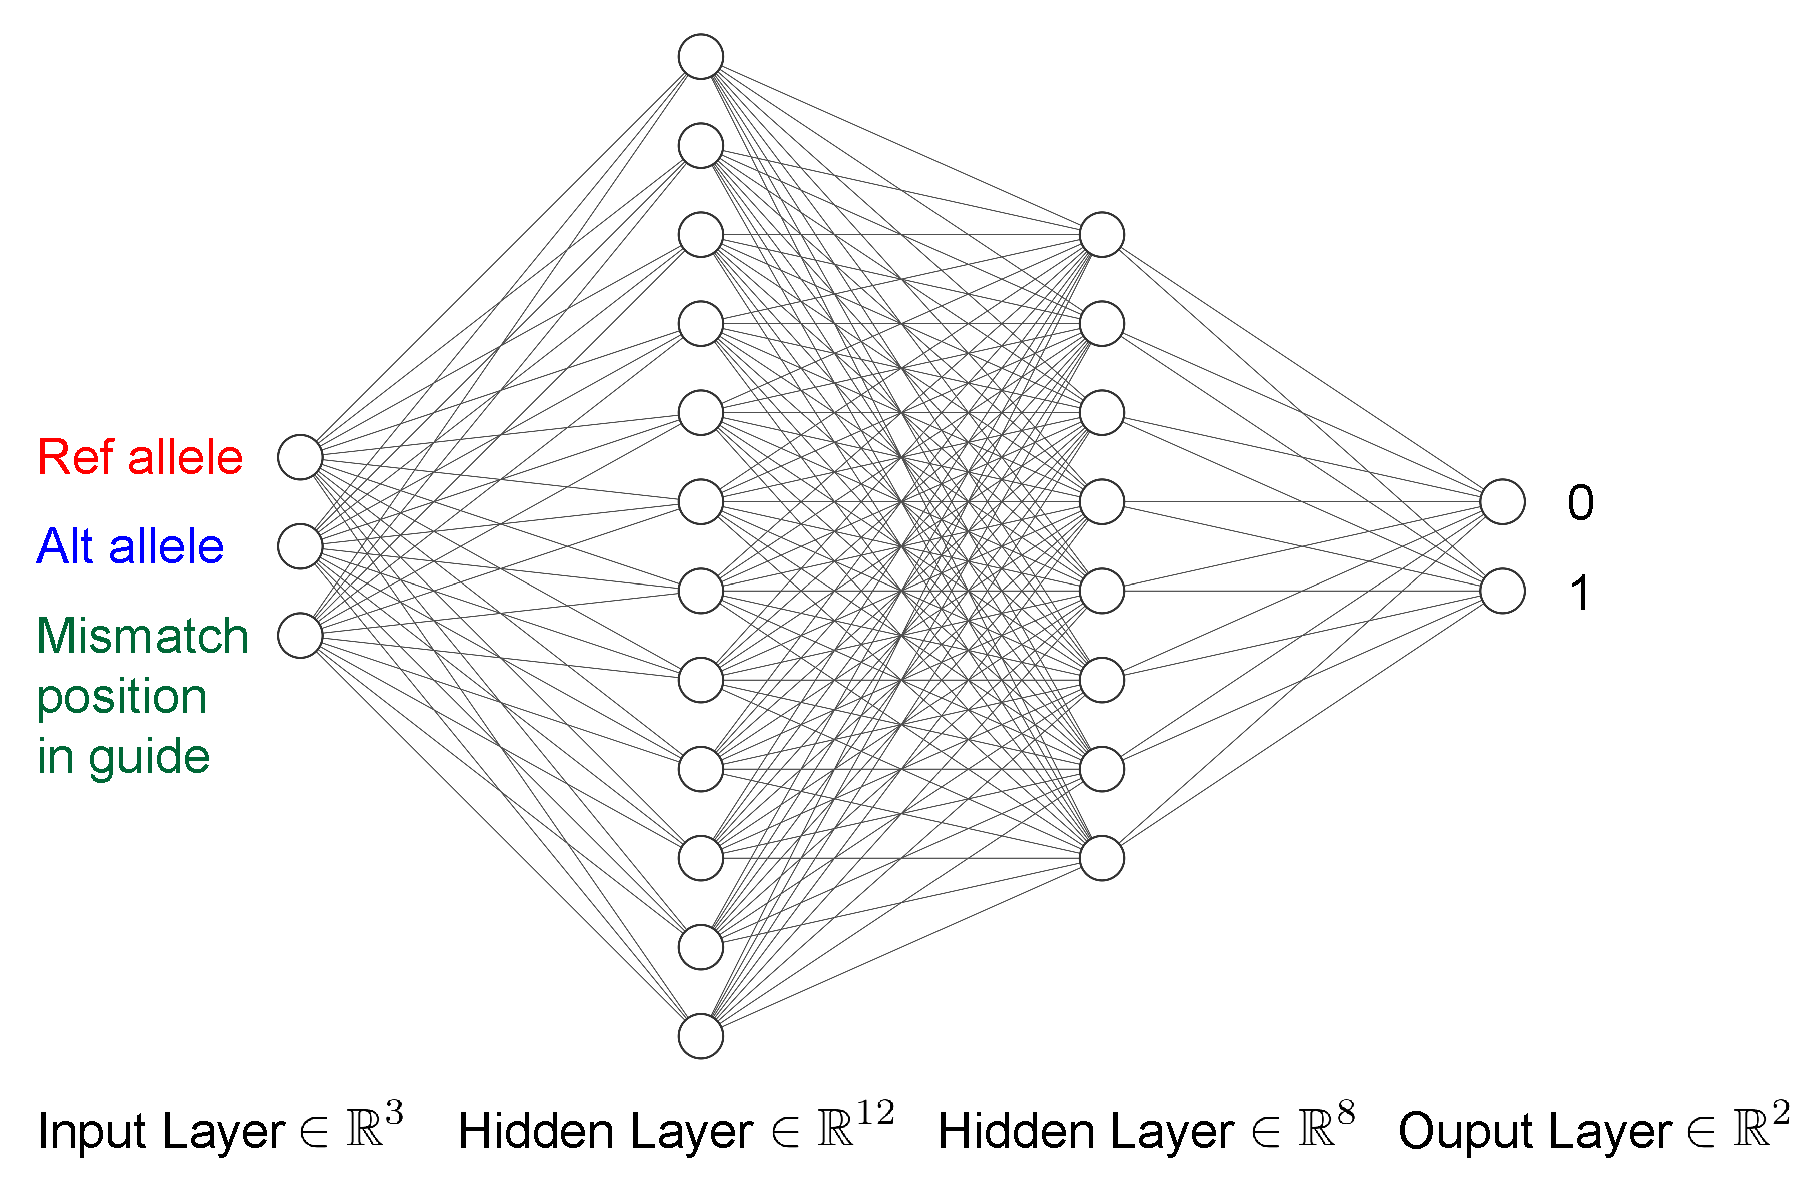
\includegraphics[width=8cm]{../NN}
		\caption{Simple DNN Structure }
	\end{center}
\end{figure}


\subparagraph*{Preprocessing}
In order to work with the DNA sequences, we used one-hot encoding from Python's SciKit Learn library to represent categorical data as binary vectors. Specifically, we converted categorical features Ref allele and Alt allele (in {A,T,C,G}) to binary vectors, and numerical feature “Mismatch position in guide” also into binary vectors (we assume every position affects Cas9 cleavage activity independently). Splitting the dataset into training the testing, there were a total of 18,717 in the training set (249 samples labeled as in-effect and 18,468 samples labeled as no-effect) 4,680 in the testing set (57 samples labeled as in-effect and 4,623 samples labeled as no-effect).

To address our imbalance classes for the training set, we implemented the SMOTE (Synthetic Minority Oversampling Technique) algorithm that creates synthetic observations of the minority class by 1). Finding the k-nearest-neighbors for minority class observations and 2). Randomly choosing one of the k-nearest neighbors to use it to create a similar but random tweaked, new observation. After preprocessing, our dataset consisted of a total of 36,856 training samples (18,468 for effect and no effect samples respectively and 4,670 testing samples. This then allowed us to identify relevant features for predicting variant fitness. We did not apply the SMOTE algorithm to the testing set. 

\textit{Logistic Regression \\ }
 Logistic regression transforms its observations to a discrete set of classe using the logistic sigmoid function to return a probability value.
\begin{align}
h_{\Theta}(X) = g(\Theta^{T} X) = g(\sum_{i=0}^{n} \theta_{i} x_{i}) \text{ where } x_0 = 1
\end{align}
 We implemented logistic regression  by using scikit.learn’s library with various C parameters. 
 
\textit{Support Vector Machine (SVM)\\}
An SVM classifies data by constructing a hyperplane with the largest margin, where the margin is the closest distance between plane and nearest points to it on either side (known as support vectors). At optimum, it becomes: 

\begin{align}
\min_{w, b, \zeta} \frac{1}{2} w^T w + C \sum_{i=1}^{n} \zeta_i
\end{aligsubject to  $y_i (w^T \phi (x_i) + b) \geq 1 - \zeta_i, & \zeta_i \geq 0, i=1, ..., n$. C, here, is a regularization parameter. The scikit.learn implementation of SVMs was used with various kenral methods. 
\begin{figure}[h]
	\begin{center} 
		\begin{subfigure}
			\centering\includegraphics[width=8cm]{../../scr/NN_Model8_Acc}
			\caption{Training and Testing Accuracy of DNN Model}
		\end{subfigure}
		\begin{subfigure}
			\centering\includegraphics[width=8cm]{../../scr/NN_Model8_Loss}
			\caption{Training and Testing Loss of DNN Model}
		\end{subfigure}
	\end{center}
\end{figure}




\textit{Random Decision Forest\\}
Random forest is another form of a supervised learning algorithm. This algorithm builds multiple decision trees and merges them together to get a more accurate and stable prediction. We chose to implement a random decision forest, because this method is highly data adaptive, applies to large a p and small n problems, and is able to account for correlation as well as interactions among features.

Begining with a binary tree, each node will split into two daughter nodes. The spliting criterion use for classification is the Gini classification. The predicted class is the most common class in the node. Therefore: 
\begin{align}
Gini = N_L \sum_{k= 1, ..., K}P_k_L(1-p_k_L) + N_r\sum_{k= 1, ..., K}p_k_R(1-p_k_R)
\end{align}
where $p_k_L$ is the proportion of class k in the left node and $p_k_R$ is the proportion of class k in the right node.  The scikit.learn implementation of random forest was used with various n-estimators. 


\textit{Neural Network (NN)\\ }
Deep learning is a class of machine learning algorithms that use multiple layers to progressively extract higher level features from raw input. The layers are made of nodes, and a node combines input from the data with sets of coefficients or weights that amplify or dampen the input by assigning the significance to inputs with regard to the task. These input weight products are summed and passed through the node’s activation function which then determines whether that signal should progress further this the network. We used a softmax cross-entropy loss, which is one of the standard loss functions for classification problems. 

\begin{align}
p_i = \sigma(s_i) = \frac{e^{s_i}}{\sum_{j = 1}^C s_j}
\end{align}
Let $y$ be the correct class. Then, the cross-entropy loss is 
\begin{align}
L = -\log p_y = -\log \left( \frac{e^{s_y}}{\sum_{j = 1}^C s_j} \right)
\end{align}
Cross-entropy loss has the advantage of being differentiable and it aims to drive all incorrect class scores to 0 while SVM loss is only concerned with increasing the correct class score above a certain margin. Our model was implemented using Keras and was trained for 30 epochs. 
\section*{Results}

\textit{Logistic Regression \\}
In our first set of experiments, we were focused on exploring the effects penalty parameter on recall score.  In these experiments, we used a penalty parameter of 0.01, 0.50, and 1.0. 

\begin{table}[h]
	\begin{center} 
		\begin{tabular}{l | c | c | c}
			Model & Test accuracy & Recall &  Precision\\ \hline \hline
			0.01, & 25 & 17.6M & 0.653 \\
			0.50 & 17 & 45.7M & 0.621 \\
			1.0 & 9 & 11.5M & 0.588 \\
		\end{tabular}
		\caption{Logistic regression metrics with varying penalty parameters.}
	\end{center}
\end{table}

The results show that the varying penalty parameter does not have a noticeable effect on recall, as all the test accuracies are within 1$\%$. Even though our accuracy score does a bit better than random guessing, changing the hyperparameters does not help increase performance.  Our highest performing accuracy is  94$\%$; however, because there is a class imbalance, although using SMOTE addresses some of the issues, the score we are hoping to be high is our recall score. The recall score here is 8.77$\%$ while the precision score is 2.20$\%$. 

\textit{Support Vector Machine\\}
Following, in our second set of experiments, we investigated the effects of kernels with an SVM. In this experiment, we used a linear kernel, polynomial kernel, radial basis function kernel, and sigmoid kernel. 
\begin{table}[h]
	\begin{center} 
		\begin{tabular}{l | c | c | c}
			Model & Test accuracy & Recall &  Precision\\ \hline \hline
			Linear & 56.58 &49.12 & 1.38 \\
			 Poly & 66.51 & 31.57& 1.16 \\
			RBF & 30.96 & 63.15& 1.10 \\
			Sigmoid & 30.72 & 63.15 & 1.105\\
		\end{tabular}
		\caption{Test accuracies of network architectures with varying kernals.}
	\end{center}
\end{table}

The results show that the kernels had a very little difference from each other. Similar to the previous experiments, the metrics are within 1 $\%$ of each other. However, unlike our first set of experiments, our accuracy performance is low but the recall score is better than random guessing being 59.64$\%$ (RBF kernel). The precision is no better than random guessing 1.10 $\%$. Refer to Figure 5 for the Confusion Matrix. 

\textit{Random Forest \\ }
The next set of experiments, we investigated if our dataset would be adaptable to random forest. This algorithm is easier to interpret in comparison to the previous algorithms, where critical features that impact classification could be readily identified and the underlying biological processes that affect biological output. We explored random forest with three different tree estimators: 10, 50, 100.
\begin{table}[h]
	\begin{center} 
		\begin{tabular}{l | c | c | c}
			Model & Test accuracy & Recall &  Precision\\ \hline \hline
			10 & 85.40 & 15.78 & 1.39 \\
			50 & 85.42 & 17.54 & 1.55 \\
			100 & 85.41 & 15.79& 1.39 \\
		\end{tabular}
		\caption{Test accuracies of network architectures with varying tree estimators.}
	\end{center}
\end{table}
 Our results show a high accuracy performance; however, the random forest model with 100 estimator performed with a 85.40 $\%$ accuracy. The recall score scored higher than our logistic regression  recall score being 15.78$\%$. However the precision score was 1.39$\%$ .  

\textit{Neural Network\\}
Our last set of experiments, we explored a DNN. We chose this method because DNNs are known to be able to better extract features and identify patterns that traditional machine learning methods may have missed. We constructed DNN used for off-target prediction consists of an input layer, two hidden layers and output layer. The input layer and the first hidden layer are both activated by a ReLu activation function. After the first input layer, there is a dropout layer with a rate of 0.25. Following the dropout layer is the second hidden layer. The second hidden layer is followed by a batch normalization layer and a dropout layer with a rate of 0.10. Proceeding that is the last hidden layer activated by a softmax activation function, with a cross-entropy is chosen as the loss function. 

\begin{table}[h]
	\begin{center} 
		\begin{tabular}{l | c | c | c}
			Model & Test accuracy & Recall &  Precision\\ \hline \hline
			Simple DNN & 62$\%$ & 37$\%$ & 1.03$\%$ \\
		\end{tabular}
		\caption{Simple DNN Metrics}
	\end{center}
\end{table}
Our DNN was able to perform with a 62$\%$  accuracy, 37$\%$  recall, and 1.03 $\%$ precision. To see our simple DNN architecture in detail refer to Figure 2.  Refer to Table V for the comparison of all the best aforementioned model’s performance. 

\section*{Discussion}


\begin{table}[h]
	\begin{center} 
		\begin{tabular}{|l|l|l|l|}
			\hline
			\textbf{Model Type}                              & \textbf{Accuracy} & \textbf{Recall} & \textbf{Precision} \\ \hline
			Logistic Regression               & \textbf{94\%}     & 8.77\%          & \textbf{2.20\%}    \\ \hline
			RBF SVM  & 30.76\%           & \textbf{64.15\%}         & 1.10\%             \\ \hline
			RF        & 85.40\%           & 15.78\%         & 1.39\%             \\ \hline
			Neural Network I  & 62\%              & 37\%            & 1.03\%             \\ \hline
		\end{tabular}
	\caption{Above is a comparison of our best performing model metrics. Each bolded score in each column highlights the highest score of all models, where our logistic regression model has the highest performing accuracy and precision score out of all the models. While our SVM model has the highest recall score out of all the other models. }
	\end{center}
	
\end{table}
There have been several scoring methods that have been used to analyze this form of data target prediction methods, such as accuracy. While we acknowledge that accuracy is important, this is misleading when the numbers of samples per class is imbalanced as well as it might conceal important information about the model fitness. Therefore, we had an emphasis on our recall metrics, rather than other metrics, because recall score is ability of a classification model to identify all relevant instances allowing for a completeness of each class. 

\textit{Traditional Machine Learning Method Comparison\\}
Overall, our logistic regression and random forest model both underperformed our SVM model. Even though our logistic regression had the highest performing accuracy of three models (94\%\). However, when examining the recall and precision score, it was worse than randomly guessing. We believe that our logistic regression algorithm may not have been be suited for our dataset. The low score in precision and recall highlights that our dataset may be unable to be linearly separable.  On the other hand, random forest, an algorithm that is typically should be adaptable to data, performed better than our logistic regression model in terms of accuracy with a score of  $85.42\%$, recall score of $17.54\%$, and a precision score of $1.55\%$. This may be due to the similarities within the dataset given little variable ranges where there may have not been many decisions trees and overfitting. However, with our SVM algorithm, our dataset may be seperated in a hyperplane allows for our dataset to be more manipulated and unconstrained. 

\begin{figure}[h]
	\begin{center} 
		\includegraphics[width=10cm]{../../scr/SVM_RBF_CM}
		\caption{From the figure, we can observe that there are $69 \%$ false positives on the effect class resulting in a  type I error. Though we have implemented SMOTE to address our imbalance classes, our new data points may be sampled from several our extreme values.}
	\end{center} 
\end{figure}

\textit{DNN Model Discussion \\}
Inspired by Lin \&\ Wong approach of their model, with a classification area of an ROC curve (AUC) of 97.2$\%$ , we wanted to also explore a DNN. Lin \&\ Wong’s dataset used a combination of multiple datasets in order to make their model (CRISPOR dataset (Tsai et al., 2015) and GUIDE-seq dataset (Jean-Paul \&\ Haeussler, M. 2018). Granted, their model was a convolutional neural network(CNN) combined with a DNN, we believed that we would be able to have a similar or better performance because the Sharon et al dataset has a more diverse set of guide RNA sequence because their dataset still had fewer positive labels when combining both dataset (143 effect from CRISPOR and 28 effect from GUIDE-seq). 

Our DNN performed with an accuracy score of  $62 \%$, recall score of $37\%$, and precision score of $1.03\%$. Examining the loss as well as the accuracy over time of the training Figure 3 and Figure 4, we observed that the rate for both is relatively steady in comparison to the testing set. For the testing set, the loss and the accuracy fluctuates. This may be due to the few samples of effect samples in the testing set or an increase amount of training time. 


\section*{Conclusion }
 Through our experiments, our SVM model had the highest recall score. Since the imbalanced nature of optimal versus sub-optimal guide RNA/donor DNA pairs means that despite moderate recall rate for prediction of test labels, we can already remove more than half of the suboptimal pairs, while still leaving sufficient guide RNA/donor DNA pairs for experiments. Most excitingly, we can start to design guide RNA/donor DNA pairs that are predicted to be optimal or suboptimal for experimental validation, to further refine our classifier.

In the future, we would also like to explore our model with additional features, such as guide RNA sequence, cutting efficiency, DNA shape, chromatin state, etc. Along with that, we would like to investigate different hyperparameters for our DNN (e.g., regularization, dropout rates, learning rante) and how the combined effort of transfer learning and DNN would better predict effect and non-effect. Having a reliable and robust model will greatly assist in better finding mutated phenotypes. 


\section*{Contributions}
Both authors contributed to this project equally. 


\section*{References}	

Chawla, N. V., Bowyer, K. W., Hall, L. O., \&\ Kegelmeyer, W. P. (2002). SMOTE: synthetic minority over-sampling technique. Journal of artificial intelligence research, 16, 321-357.

Chuai, G., Ma, H., Yan, J., Chen, M., Hong, N., Xue, D., Zhou, C., Zhu, C., Chen, K., Duan, B., et al.(2018). DeepCRISPR: optimized CRISPR guide RNA design by deep learning. Genome Biol. 19, 80.

He, K., Zhang, X., Ren, S., \&\ Sun, J. (2016). Deep residual learning for image recognition. In Proceedings of the IEEE conference on computer vision and pattern recognition (pp. 770-778).

Jean-Paul, C. \&\ Haeussler, M. (2018). CRISPOR: intuitive guide selection for CRISPR/Cas9 genome editing experiments and screens. Nucleic Acids Res. 46, W242–W245.

Krizhevsky, A., Sutskever, I., \&\ Hinton, G. E. (2012). Imagenet classification with deep convolutional neural networks. In Advances in neural information processing systems (pp. 1097-1105).

Lin, J., Wong, K.-C. (2018). Off-target predictions in CRISPR-Cas9 gene editing using deep learning. Bioinformatics. 34, i656–i663.

Sharon, E., Chen, S. A. A., Khosla, N. M., Smith, J. D., Pritchard, J. K., \&\ Fraser, H. B. (2018). Functional genetic variants revealed by massively parallel precise genome editing. Cell, 175(2), 544-557

Tsai, S.Q., Zheng, Z., Nguyen, N.T., Liebers, M., Topkar, V.V., Thapar, V., Wyvekens, N., Khayter, C., Iafrate, A.J., Le, L.P., et al. (2015). GUIDE-seq enables genome-wide profiling of off-target cleavage by CRISPR-Cas nucleases. Nat. Biotech. 33, 187–197.


\end{document}
